\markboth{Exploring Android Stack}{Introduction}

\section{Introduction}
In 2011, 48.8\% of the smartphones on the market, ran Android OS, contributing to an annual growth of 244\%.\footnote{Source: Canalys. February 2012} This is what an average customer can easily guess by himself. What not everyone can figure, unless he's working in this very specific field, is that lately Android OS - and therefore its open source project AOSP - aroused the curiosity of many embedded developers.\\
As we can see in Fig. \ref{fig:stack} \cite{gargenta}, Andrdoid's architecture can be divided into many components, which we'll briefly analyse - following a bottom-up approach - before going deeper into the core of this work.
\begin{figure}[!htb]
	\centering
	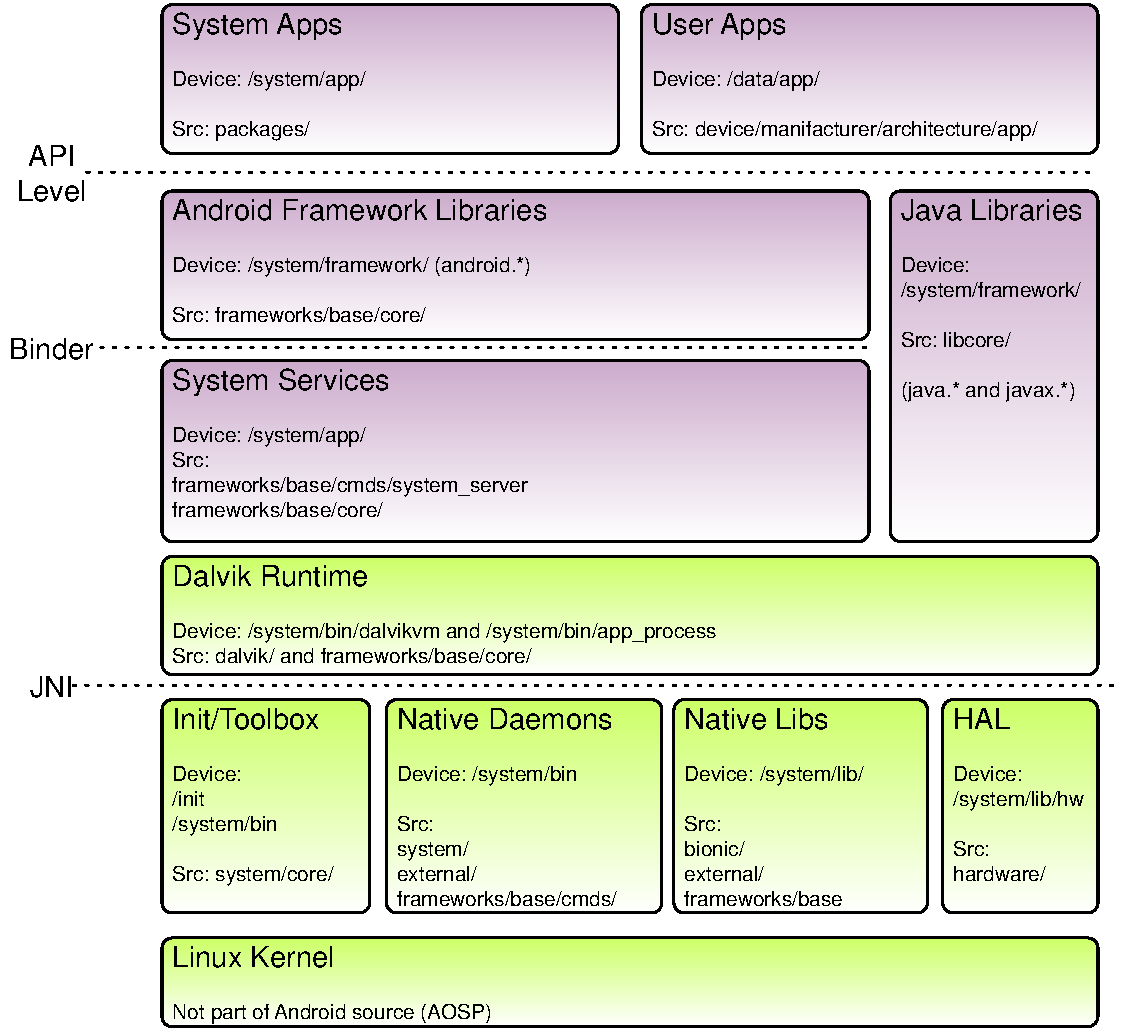
\includegraphics[scale=.6]{images/stack.pdf}
	\caption{Android's stack}
	\label{fig:stack}
\end{figure}
\begin{itemize}
\item \textbf{Linux Kernel}\\
Android kernels are, in sum, forks from the mainline kernel, relying on several custom 	functionalities that are significantly different from what is found in the "vanilla" kernel. Follows a brief enumeration of the most remarkable customizations made to the kernel to satisfy special Android's needs.
	\begin{itemize}
	\item \textsc{Wakelocks}\\
	Instead of letting the system be put to sleep at the user's behest, an "Androidized"
kernel is made to go to sleep as soon and as often as possible. \textit{Wakelocks} are provided to keep the system awake while performing specific processing. The wakelocks and early suspend functionality are actually built on top of Linux's existing power management functionality.
	\item \textsc{Low Memory Killer (LMK)}\\
	Since Android system tipically runs in low-memory conditions, the \textit{out-of-memory} (OOM) handling is crucial: therefore the Android development team has introduced an additional \textit{LMK} - based on priorities to identify \textit{to-be-killed} candidates - that kicks in just before the default kernel OOM killer does (thus preempting its intervention, which occurs only when no memory is left).
	\item \textsc{Binder}\\
	Binder allows apps to talk the System Server and it's what apps use to talk to each others' service components, although they actually perform this communication through  interfaces and stubs generated by the \textit{aidl} tool. In Fig. \ref{fig:binder_flow} and example of the communication flow: the Activity (which is what we're used to call "App", despite this word in the Android Framework acquires different meanings) requires to the \textit{Service Manager} an instance of a specific Service she wants to interact with, and performs this operation through \textit{Stubs} and \textit{Binder}.
		\begin{figure}[!htb]
			\centering
			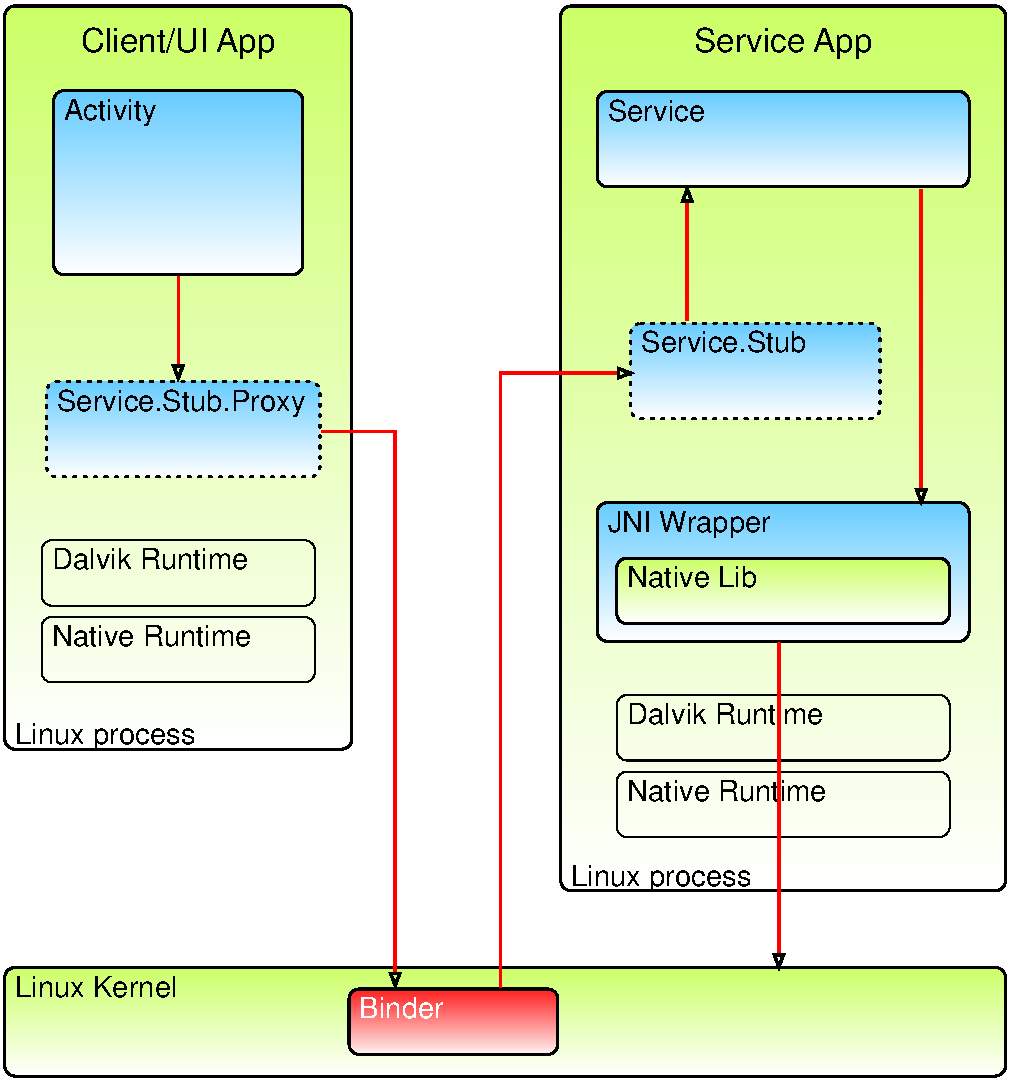
\includegraphics[scale=.4]{images/binder_flow.pdf}
			\caption{Communication Activity-Service through Binder}
			\label{fig:binder_flow}
		\end{figure}
	\item \textsc{Anonymous Shared Memory}\\
	Typically, a first process creates a shared memory region using \textit{ashmem} and uses Binder to share the corresponding file descriptor with other processes with which it wishes to share the region. \textit{Ashmem} destroys memory regions when all processes referring to them have exited and will shrink mapped regions if the system is in need of memory.
	\item \textsc{Alarm}\\
	Android's alarm driver is actually layered on top of the kernel's existing Real-Time Clock (RTC) and High-Resolution Timers (HRT) functionalities. Android's alarm driver cleverly combines the best of both worlds: by default the driver uses the kernel's High-Resolution Timer (HRT) functionality, but whenever the system is about to suspend itself, it programs the RTC so that the system gets woken up at the appropriate time.
	\item \textsc{Logger}\\
	Logger
	\end{itemize}
\end{itemize}